\definecolor{tableheadercolor}{HTML}{3aa827}
\chapter{rogettazione logica}
\section{Stima del volume dei dati}
\begin{table}[H]
  \centering
  \rowcolors{2}{green!80!black!40}{white}
  \begin{tabular}{ccc}
    \rowcolor{tableheadercolor}
    \textbf{Concetto} & \textbf{Costrutto} & \textbf{Volume} \\
    Centri & E & 84 \\
    Posizioni & E & 166 \\
    Settori & E & 125 \\
    Controllori & E & 4200 \\
    Ferie & E & 8400 \\
    Abilitazione & E & 4200 \\
    Turni (mensili) & E & 20000 \\
    Aerodromi & E & 43 \\
    Piste & E & 43 \\
    Punti & E & 3750 \\
    Piani di volo (mensili) & E & 5000 \\
    Aereomobili & E & 5000 \\
    Composizione (settori postazioni) & R & 125 \\
    Abilitamento (abilitazioni settori) & R & 4200 \\
    Stimati & R & 500.000 \\
    Percorrenza & R & 500.000 \\
  \end{tabular}
  \end{table}
  \section{Descrizione delle operazioni principali e stima della loro frequenza}

  \begin{table}[H]
  \centering
  \rowcolors{2}{green!80!black!40}{white}
  \begin{tabular}{ccc}
  \rowcolor{tableheadercolor}
  \textbf{Codice} & \textbf{Operazione} & \textbf{Frequenza stimata} \\

  OP1 & Aggiunta e/o rimozione di un nuovo controllore di volo & 3 al mese \\
  OP2 & Modifica dei dati personali di un controllore di volo & 10 al mese \\
  OP3 & Assegnazione delle ferie a un controllore di volo & 100 al mese \\
  OP4 & Aggiunta di un'abilitazione a un controllore di volo & 50 al mese \\
  OP5 & Calcolo dei turni mensili per i controllori di volo & 1 al mese \\
  OP6 & Aggiunta di un nuovo piano di volo & 2000 al mese \\
  OP7 & Rimozione di un piano di volo & 100 al mese \\
  OP8 & Modifica di un piano di volo esistente & 1500 al mese \\
  OP9 & Aggiunta e/o rimozione di un nuovo aereomobile & 50 al mese \\
  OP10 & Calcolo del ral & 1 all'anno \\
  OP11 & Stima dei voli in un settore in un ora & 500.000 al mese \\
  OP12 & Aggiunta di una percorrenza & 500.000 al mese \\


  \end{tabular}
  \end{table}
  
  La tabella sopra riportata fornisce un elenco delle operazioni principali che possono essere eseguite nel sistema di gestione del personale di controllo del traffico aereo. Per ciascuna operazione, viene fornita una stima numerica della loro frequenza stimata al mese.
\section{Schemi di navigazione e tabelle degli accessi}
Sono riportate in seguito le tabelle degli accessi delle operazioni sopra riportate, inoltre, ove
non risulti banale, sono stati inseriti i relativi schemi di navigazione. Al fine del calcolo degli
costi, si considerano di peso doppio gli accessi in scrittura rispetto a quelli in lettura.

\subsection*{OP1 - Modifica dei dati personali di un controllore di volo}
\begin{table}[H]
  \centering
  \rowcolors{2}{green!80!black!40}{white}
  \begin{tabular}{cccc}

  \rowcolor{tableheadercolor}
  \textbf{Concetto} & \textbf{Costrutto} & \textbf{accessi} & \textbf{tipo}\\

  Controllore & E & 1 & S \\
  &  & Totale: 1S, 6 al mese &\\

  \end{tabular}
  \end{table}

    \subsection*{OP2 - Modifica dei dati personali di un controllore di volo}
    \begin{table}[H]
      \centering
      \rowcolors{2}{green!80!black!40}{white}
      \begin{tabular}{cccc}
    
      \rowcolor{tableheadercolor}
      \textbf{Concetto} & \textbf{Costrutto} & \textbf{accessi} & \textbf{tipo}\\
    
      Controllore & E & 1 & L \\
      Controllore & E & 1 & S \\
      &  & Totale: 1S 1L, 30 al mese &\\
    
      \end{tabular}
      \end{table}
  
      \subsection*{OP3 - Assegnazione delle ferie a un controllore di volo}
      \begin{table}[H]
    \centering
    \rowcolors{2}{green!80!black!40}{white}
    \begin{tabular}{cccc}
  
    \rowcolor{tableheadercolor}
    \textbf{Concetto} & \textbf{Costrutto} & \textbf{accessi} & \textbf{tipo}\\
  
    Controllore & E & 1 & L \\
    Ferie & E & 1 & S \\
    & & Totale: 1S, 1L, 300 al mese &\\
  
    \end{tabular}
    \end{table}

    \subsection*{OP4 - Aggiunta di un'abilitazione a un controllore di volo}
    \begin{table}[H]
    \centering
    \rowcolors{2}{green!80!black!40}{white}
    \begin{tabular}{cccc}
  
    \rowcolor{tableheadercolor}
    \textbf{Concetto} & \textbf{Costrutto} & \textbf{accessi} & \textbf{tipo}\\
  
    Controllore & E & 1 & L \\
    Abilitamento & R & 1 & S \\
    Abilitazione & E & 1 & S \\
    & & Totale: 2S, 1L, 250 al mese &\\
  
    \end{tabular}
    \end{table}

    \subsection*{OP5 - Calcolo dei turni mensili per i controllori di volo}
    \begin{table}[H]
    \centering
    \rowcolors{2}{green!80!black!40}{white}
    \begin{tabular}{cccc}
  
    \rowcolor{tableheadercolor}
    \textbf{Concetto} & \textbf{Costrutto} & \textbf{accessi} & \textbf{tipo}\\
  
    Controllore & E & 4200 & L \\
    Turno & E & 20000 & L \\
    Stimato & E & 500.000 & L \\
    Postazione & E & 166 & L \\
    Settore & E & 125 & L \\
    & & Totale: 0S, 524,491L, 524.491 al mese &\\
  
    \end{tabular}
    \end{table}
    Per ogni turno e per ogni posizione viene calcolata l'occupazione e viene cercato il controllore adatto con meno turni lavorati.
    Il modo con cui conteggiamo le letture non tiene conto delle ricerche, l'operazine effettiva sul calcolatore è estremamente pesante.
    \begin{figure}[H]
      \centering
      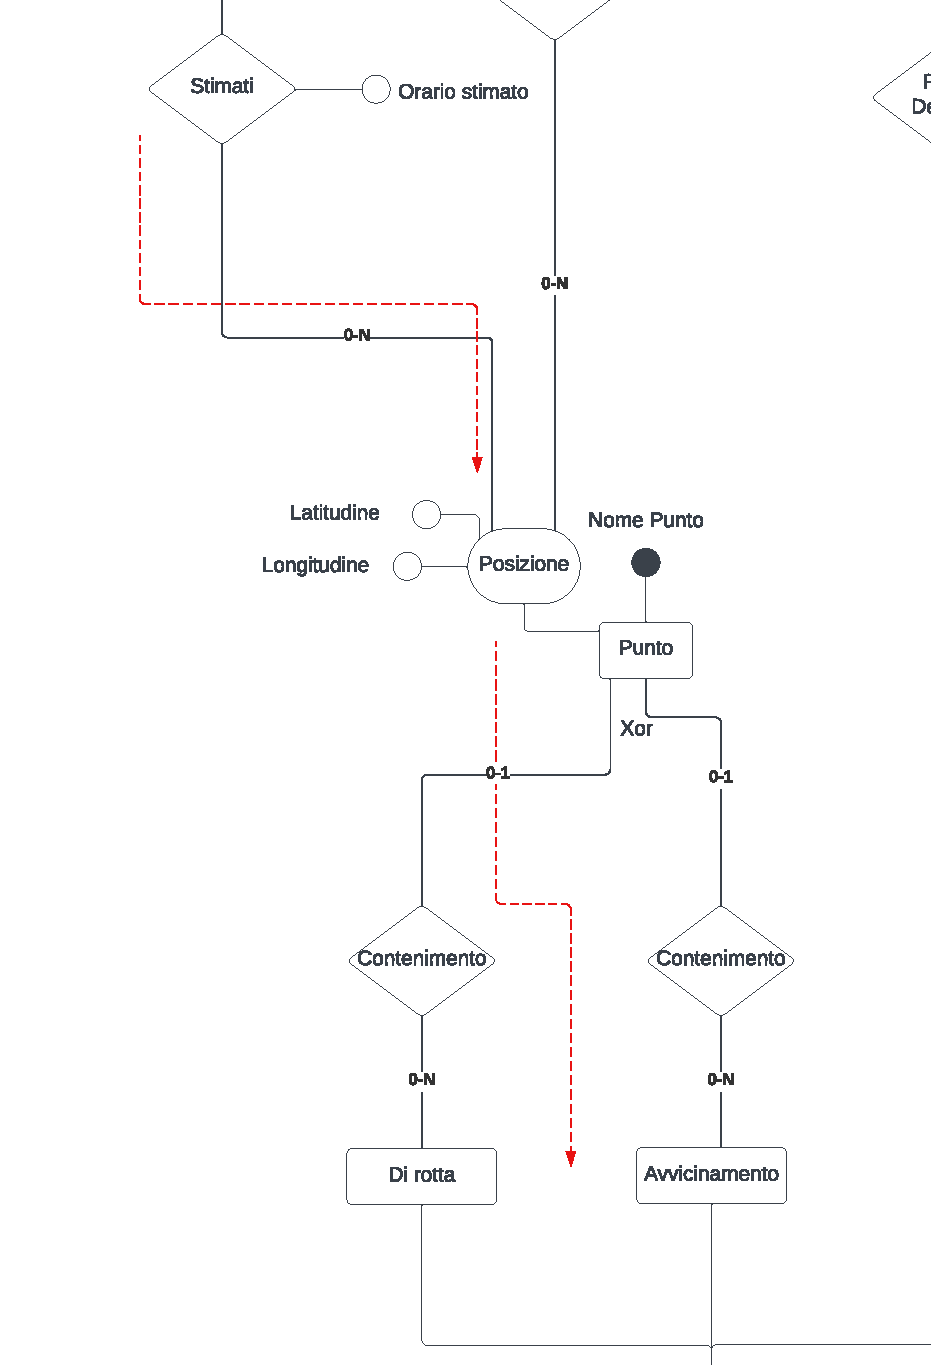
\includegraphics[width=10cm]{figures/BasicControllerarrowsp1.pdf}
      \caption{"Percorso per trovare l'occupazione"}
    \end{figure}
    \begin{figure}[H]
      \centering
      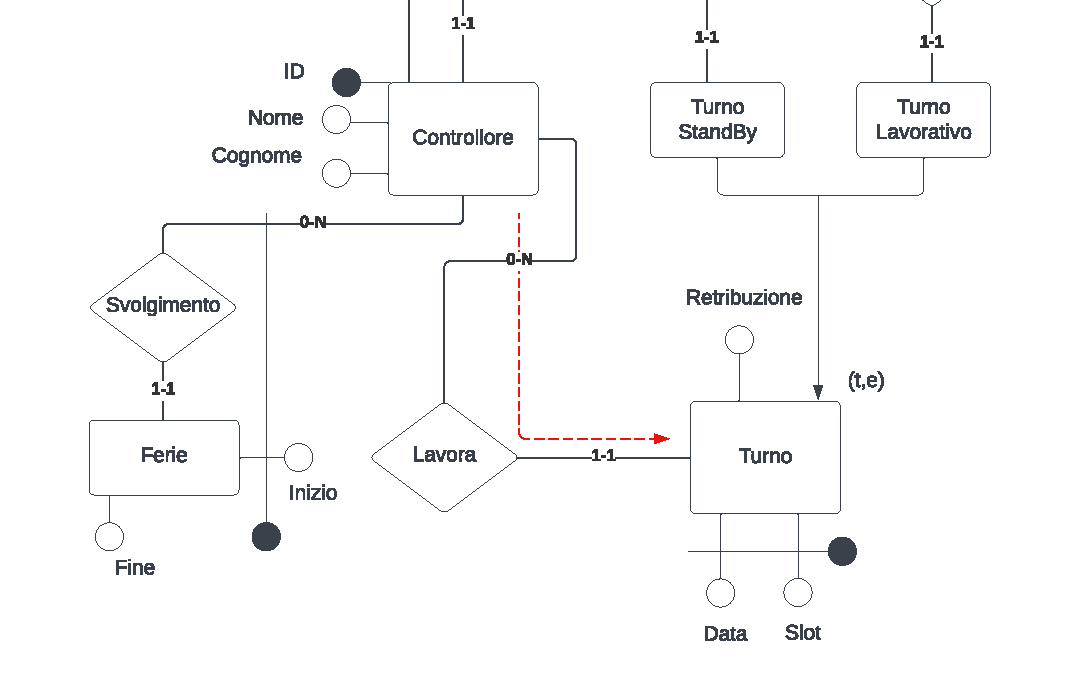
\includegraphics[width=1\textwidth]{figures/BasicControllerarrowsp2.pdf}
      \caption{"Percorso per trovare I turni lavorati"}
    \end{figure}

    \subsection*{OP6 - Aggiunta di un nuovo piano di volo}
    \begin{table}[H]
    \centering
    \rowcolors{2}{green!80!black!40}{white}
    \begin{tabular}{cccc}
  
    \rowcolor{tableheadercolor}
    \textbf{Concetto} & \textbf{Costrutto} & \textbf{accessi} & \textbf{tipo}\\
  
    Piano di Volo & E & 1 & S \\
    Stimati & E & 100 & S \\
    Punti & E & 100 & R \\
    Piste & E & 2 & R \\
    Aereomobile & E & 1 & R \\
    & & Totale: 101S, 103L, 610.000 al mese &\\
  
    \end{tabular}
    \end{table}

    \subsection*{OP7 - Aggiunta di un nuovo piano di volo}
    \begin{table}[H]
    \centering
    \rowcolors{2}{green!80!black!40}{white}
    \begin{tabular}{cccc}
  
    \rowcolor{tableheadercolor}
    \textbf{Concetto} & \textbf{Costrutto} & \textbf{accessi} & \textbf{tipo}\\
  
    Piano di Volo & E & 1 & S \\
    Stimati & E & 100 & S \\
    Punti & E & 100 & R \\
    Piste & E & 2 & R \\
    Aereomobile & E & 1 & R \\
    & & Totale: 101S, 103L, 30.500 al mese &\\
  
    \end{tabular}
    \end{table}
  
    \subsection*{OP8 - Modifica di un piano di volo esistente}
    \begin{table}[H]
    \centering
    \rowcolors{2}{green!80!black!40}{white}
    \begin{tabular}{cccc}
  
    \rowcolor{tableheadercolor}
    \textbf{Concetto} & \textbf{Costrutto} & \textbf{accessi} & \textbf{tipo}\\
  
    Piano di Volo & E & 1 & S \\\
    & & Totale: 1S, 0L, 3.000 al mese &\\
  
    \end{tabular}
    \end{table}

    \subsection*{OP9 - Aggiunta e/o rimozione di un nuovo aereomobile}
    \begin{table}[H]
    \centering
    \rowcolors{2}{green!80!black!40}{white}
    \begin{tabular}{cccc}
  
    \rowcolor{tableheadercolor}
    \textbf{Concetto} & \textbf{Costrutto} & \textbf{accessi} & \textbf{tipo}\\
  
    Aereomobile & E & 1 & S \\\
    & & Totale: 1S, 0L, 100 al mese &\\
  
    \end{tabular}
    \end{table}

    \subsection*{OP10 - Calcolo del ral}
    \begin{table}[H]
    \centering
    \rowcolors{2}{green!80!black!40}{white}
    \begin{tabular}{cccc}
  
    \rowcolor{tableheadercolor}
    \textbf{Concetto} & \textbf{Costrutto} & \textbf{accessi} & \textbf{tipo}\\
  
    Controllore & E & 4200 & L \\
    Turno & E & 240.000 & L \\
    & & Totale: 0S, 244.200L, 20.000 al mese &\\
  
    \end{tabular}
    \end{table}
  
    \subsection*{OP11 - Stima dei voli in un settore in un ora}
    \begin{table}[H]
    \centering
    \rowcolors{2}{green!80!black!40}{white}
    \begin{tabular}{cccc}
  
    \rowcolor{tableheadercolor}
    \textbf{Concetto} & \textbf{Costrutto} & \textbf{accessi} & \textbf{tipo}\\
  
    Stimato & E & 30 & L \\
    Postazione & E & 1 & L \\
    Settore & E & 2 & L \\
    & & Totale: 0S, 33L, 16.500.000 al mese &\\
  
    \end{tabular}
    \end{table}
    \begin{figure}[H]
      \centering
      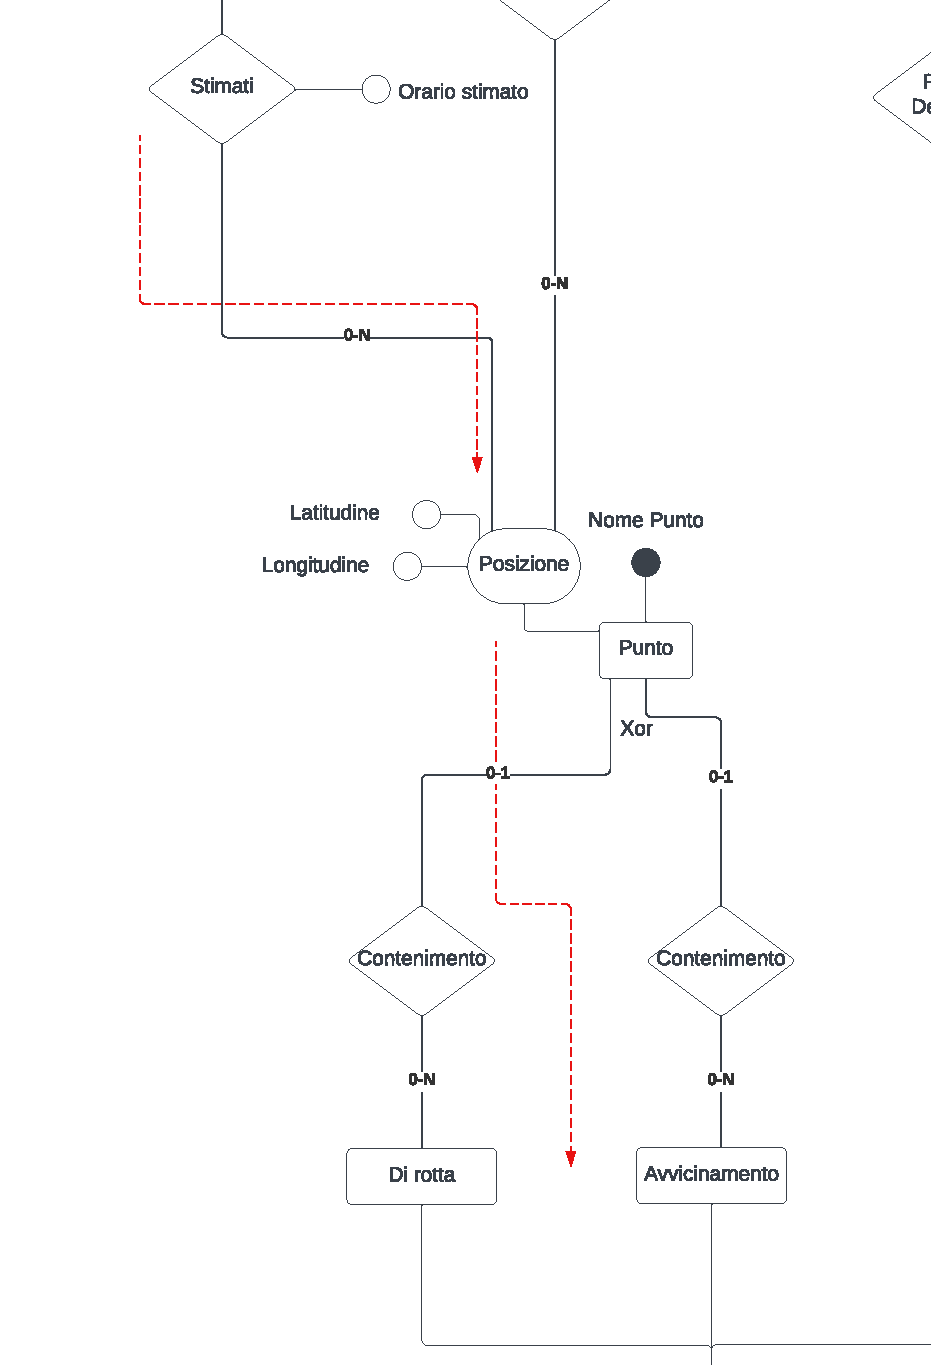
\includegraphics[width=10cm]{figures/BasicControllerarrowsp1.pdf}
      \caption{"Percorso per trovare l'occupazione"}
    \end{figure}
    
    \subsection*{OP11 - Aggiunta di una percorrenza}
    \begin{table}[H]
    \centering
    \rowcolors{2}{green!80!black!40}{white}
    \begin{tabular}{cccc}
  
    \rowcolor{tableheadercolor}
    \textbf{Concetto} & \textbf{Costrutto} & \textbf{accessi} & \textbf{tipo}\\
  
    Percorrenza & E & 1 & S \\\
    & & Totale: 1S, 0L, 1.000.000 al mese &\\
  
    \end{tabular}
    \end{table}
  
\section{Raffinamento dello schema}
\subsection*{Eliminazione delle gerarchie}
In questo caso è stato adottato un collasso verso il basso separando i turni lavorativi da quelli standby. 
Stessa Cosa è stata fatta per i tipi di postazione, anche se quella "avvicinamento" e "di rotta" sono state unite in un'unica in quanto ai fini dell'architettura logica non vi sono differenze.


\subsection*{Eliminazione degli attributi compositi}
Gli attributi composti di posizione sono stati eliminati creando gli attributi longitudine e latitudine direttamente nelle entità.
\subsection*{Eliminazione degli identificatori esterni}
Si sono risolti rimuovendo le assciazioni in quanto risultavano di tipo 1-1.
\section{Analisi delle ridondanze}
In questa sezione calcoleremo se è conveniente inserire un attributo guadagni all'entità controllore al fine di calcolare il reddito annuale (OP10):\\
Nel caso con ridondanza l'attributo verrebbe aggiornato ogni volta che viene inserito un turno per poi eseguire un unica lettura a fine anno.
\begin{table}[H]
     \centering
     \rowcolors{2}{green!80!black!40}{white}
     \begin{tabular}{cccc}
   
     \rowcolor{tableheadercolor}
     \textbf{Concetto} & \textbf{Costrutto} & \textbf{accessi} & \textbf{tipo}\\
   
     controllore & E & 300 & S \\
     controllore & E & 1 & L \\
     & & Totale: 300S, 1L, 601 all'anno &\\
   
     \end{tabular}
     \end{table}
Nel caso senza ridondanza bisogna leggere tutti i turni svolti nell'anno e sommare i guadagni:
\begin{table}[H]
     \centering
     \rowcolors{2}{green!80!black!40}{white}
     \begin{tabular}{cccc}
   
     \rowcolor{tableheadercolor}
     \textbf{Concetto} & \textbf{Costrutto} & \textbf{accessi} & \textbf{tipo}\\
   
     turni & E & 300 & L \\
     & & Totale: 0S, 300L, 300 all'anno &\\
   
     \end{tabular}
     \end{table}

Chiaramente il secondo caso è più conveniente, si procederà quindi senza ridondanze.


\section{Traduzione di entità e associazioni in relazioni}
Tutte le realzioni sono state spostate dentro le entità, in quanto la maggior parte erano di tipo 1-1 o 0-1,
sono invece state create nuove entità:
\begin{itemize}
  \item Composizione settori, per salvare da quali settori sono composte le postazioni.
  \item Abilitazione settori, per salvare quali settori abilitano le relative abilitazioni.
  \item Stimati, per salvare l'orario stimato su un punto.
  \item Percorrenza, per salvare l'orario di sorvolo su un punto.
\end{itemize}

Abilitazione (
     MatricolaAbilitazione,
     IdControllore,
     primary key (MatricolaAbilitazione))\\

AbilitazioneSettori (
     MatricolaAbilitazione,
     IdSettore,
     primary key (MatricolaAbilitazione, IdSettore))\\

Aereomobile (
     Tipo,
     NumeroDiCoda,
     primary key (NumeroDiCoda))\\

Aerodromo (
     AdLatitudine,
     AdLongitudine,
     CodiceIcao,
     CodiceIata,
     primary key (CodiceIcao))\\

Centro (
     NomeCentro,
     primary key (NomeCentro))\\

ComposizioneSettori (
     IdPostazione,
     IdSettore,
     primary key (IdPostazione, IdSettore))\\

Controllore (
     IdControllore,
     Nome,
     Cognome,
     NomeCentro,
     primary key (IdControllore))\\

Ferie (
     IdControllore,
     Inizio,
     Fine,
     primary key (IdControllore, Inizio))\\

Percorrenza (
     Callsign,
     Dof,
     NomePunto,
     OrarioDiSorvolo,
     primary key (Callsign, Dof, NomePunto))\\

PianoDiVolo (
     OrarioAtterraggio*,
     OrarioDecollo*,
     Callsign,
     Dof,
     NumeroDiCoda,
     CodAdDecollo,
     OrientamentoPistaDecollo,
     CodAdAtterraggio,
     OrientamentoPistaAtterraggio,
     primary key (Callsign, Dof))\\

Pista (
     CodAd,
     Orientamento,
     Lunghezza,
     primary key (CodAd, Orientamento))\\

Postazione (
     IdPostazione,
     NomeCentro,
     primary key (IdPostazione))\\

Punto (
     NomePunto,
     PosLatitudine,
     PosLongitudine,
     IdSettore,
     primary key (NomePunto))\\

Settore (
     IdSettore,
     CodAd,
     primary key (IdSettore))\\

Stimati (
     Callsign,
     Dof date,
     NomePunto,
     OrarioStimato,
     primary key (Callsign, Dof, NomePunto))\\

Turno (
     IdControllore,
     Retribuzione,
     Data,
     Slot,
     IdPostazione*,
     CentroStandBy*,
     primary key (IdControllore, Data, Slot))\\
\section{Schema relazionale finale}
\begin{figure}[H]
  \centering
  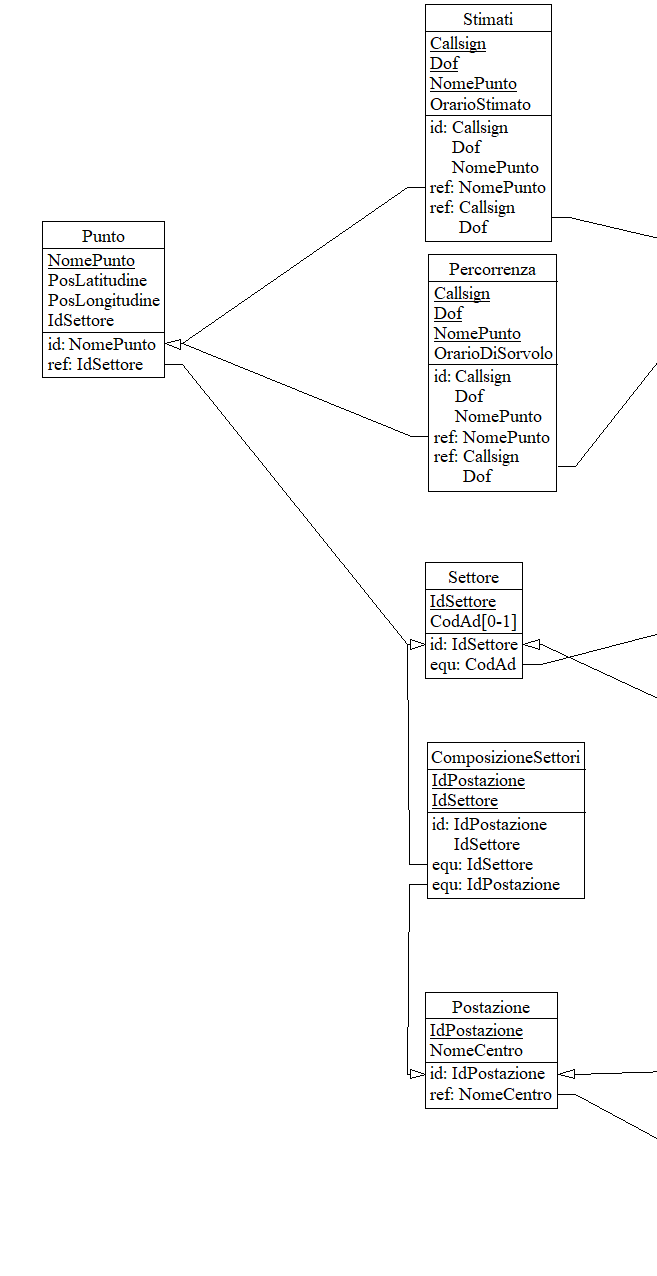
\includegraphics[height=1\textheight]{figures/Capture1.PNG}
  \caption{"Schema sinistro della relazionale finale"}
\end{figure}
\begin{figure}[H]
  \centering
  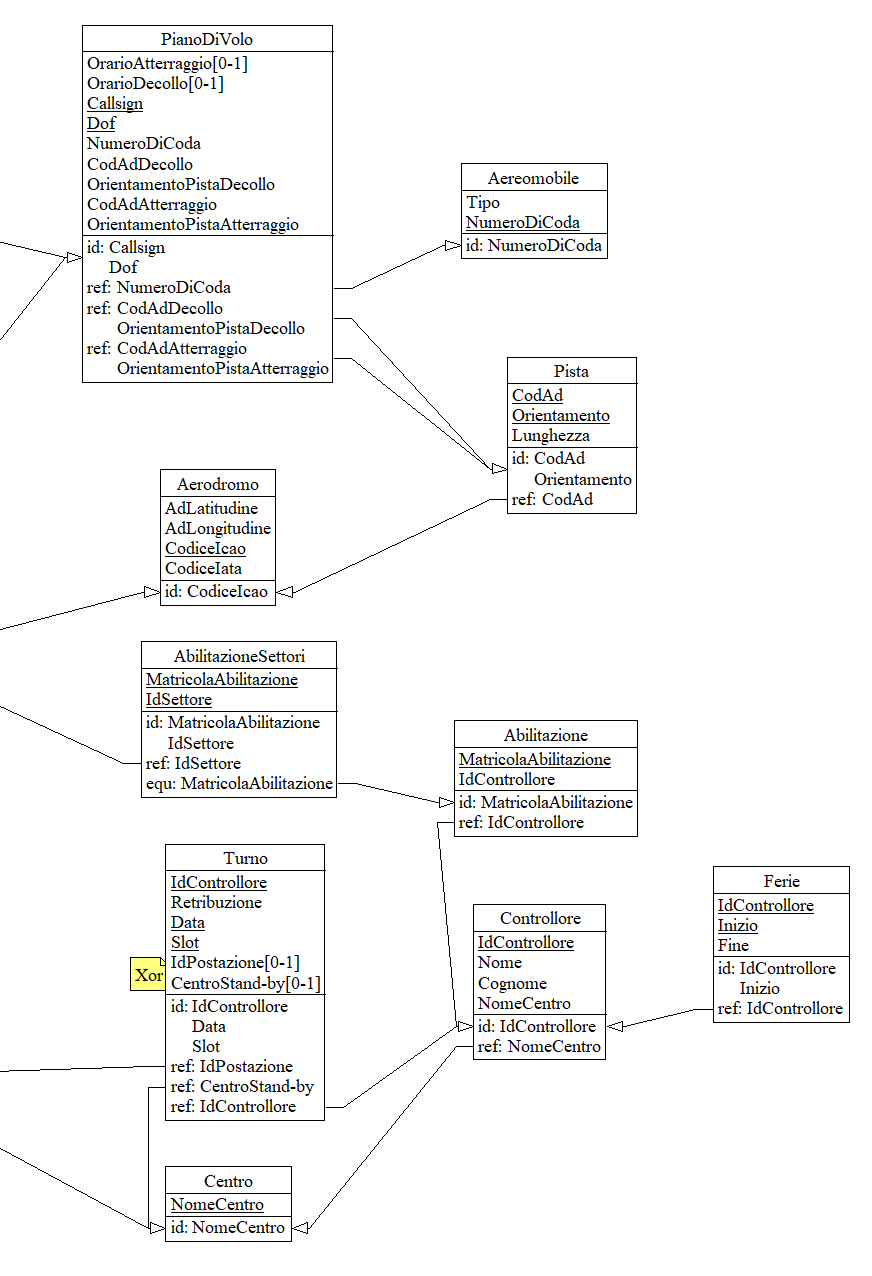
\includegraphics[width=1\textwidth]{figures/Capture2.PNG}
  \caption{"Schema destro della relazionale finale"}
\end{figure}
\section{Traduzione delle operazioni in query SQL}
% Define colors
\definecolor{sqlKeywords}{RGB}{0,0,255}
\definecolor{sqlStrings}{RGB}{163,21,21}
\definecolor{sqlComments}{RGB}{0,128,0}

% Define SQL style
\lstdefinestyle{sqlStyle}{
  language=SQL,
  basicstyle=\small\ttfamily,
  keywordstyle=\color{sqlKeywords},
  stringstyle=\color{sqlStrings},
  commentstyle=\color{sqlComments},
  breaklines=true,
  showstringspaces=false,
  numbers=left,
  numberstyle=\tiny\color{gray},
  frame=single,
  captionpos=b
}
\lstset{style=sqlStyle}

\section*{SQL Queries}

OP1 - Aggiunta e/o rimozione di un nuovo controllore di volo:
\begin{lstlisting}
-- Aggiunta di un nuovo controllore di volo
INSERT INTO Controllore (IdControllore, Nome, Cognome, NomeCentro)
VALUES ('nuovo_id', 'Nuovo Nome', 'Nuovo Cognome', 'Nome Centro');

-- Rimozione di un controllore di volo
DELETE FROM Controllore
WHERE IdControllore = 'id_controllore_da_rimuovere';
\end{lstlisting}

OP2 - Modifica dei dati personali di un controllore di volo:
\begin{lstlisting}
UPDATE Controllore
SET Nome = 'Nuovo Nome', Cognome = 'Nuovo Cognome'
WHERE IdControllore = 'id_controllore_da_modificare';
\end{lstlisting}

OP3 - Assegnazione delle ferie a un controllore di volo:
\begin{lstlisting}
-- Aggiunta delle ferie
INSERT INTO Ferie (IdControllore, Inizio, Fine)
VALUES ('id_controllore', 'data_inizio_ferie', 'data_fine_ferie');

-- Rimozione delle ferie
DELETE FROM Ferie
WHERE IdControllore = 'id_controllore' AND Inizio = 'data_inizio_ferie';
\end{lstlisting}

OP4 - Aggiunta di un'abilitazione a un controllore di volo:
\begin{lstlisting}
INSERT INTO Abilitazione (MatricolaAbilitazione, IdControllore)
VALUES (nuova_matricola, 'id_controllore');

INSERT INTO AbilitazioneSettori (MatricolaAbilitazione, IdSettore)
VALUES (nuova_matricola, 'id_settore');
\end{lstlisting}

OP5 - Calcolo dei turni mensili per i controllori di volo:
Sarebbe estremamanete complicato riassumere questa operzione in un unica query, se il lettore è interessato può esamiare il codice dell'applicativo che utilizza un ORM.

OP6 - Aggiunta di un nuovo piano di volo:
\begin{lstlisting}
INSERT INTO PianoDiVolo (OrarioAtterraggio, OrarioDecollo, Callsign, Dof, NumeroDiCoda, CodAdDecollo, OrientamentoPistaDecollo, CodAdAtterraggio, OrientamentoPistaAtterraggio)
VALUES ('data_atterraggio', 'data_decollo', 'callsign', 'data', 'numero_coda', 'cod_ad_decollo', 'orientamento_decollo', 'cod_ad_atterraggio', 'orientamento_atterraggio');
\end{lstlisting}

OP7 - Rimozione di un nuovo piano di volo:
\begin{lstlisting}
DELETE FROM PianoDiVolo
WHERE dof = 'dof' and callsign = 'callsign';
\end{lstlisting}

OP8 - Modifica di un nuovo piano di volo esistente:
\begin{lstlisting}
UPDATE PianoDiVolo (OrarioAtterraggio, OrarioDecollo, Callsign, Dof, NumeroDiCoda, CodAdDecollo, OrientamentoPistaDecollo, CodAdAtterraggio, OrientamentoPistaAtterraggio)
SET OrarioAtterraggio = 'data_atterraggio', OrarioDecollo = 'data_decollo', NumeroDiCoda = 'numero_coda', CodAdDecollo = 'cod_ad_decollo', OrientamentoPistaDecollo = 'orientamento_decollo', CodAdAtterraggio = 'cod_ad_atterraggio', OrientamentoPistaAtterraggio = 'orientamento_atterraggio'
WHERE dof = 'dof' and callsign = 'callsign';

\end{lstlisting}

OP9 - Aggiunta e/o rimozione di un nuovo aereomobile:
\begin{lstlisting}
     -- Aggiunta nuovo Aereomobile
     INSERT INTO Aereomobile (NumeroDiCoda, NumeroDiCoda)
     VALUES ('NumeroDiCoda', 'NumeroDiCoda');
     
     -- Rimozione delle ferie
     DELETE FROM Aereomobile
     WHERE NumeroDiCoda = 'NumeroDiCoda';
     \end{lstlisting}

OP10 - Calcolo del reddito annuo lordo di un controllore di volo:
\begin{lstlisting}
SELECT sum(Retribuzione) FROM turno
where year(data) = 'anno' and IdControllore='id controllore';
\end{lstlisting}

OP11 - Stima dei voli in un settore in un'ora:
\begin{lstlisting}
     select * FROM atctables.stimati s, atctables.punto p
     WHERE p.NomePunto = s.NomePunto AND
     Dof = 'data' AND OriarioStimato BETWEEN 'ora_inizio' AND 'ora_fine' AND IdSettore = 'idSettore';
\end{lstlisting}

OP12 - Aggiunta di una percorrenza:
\begin{lstlisting}
INSERT INTO Percorrenza (Callsign, Dof, NomePunto, OrarioDiSorvolo)
VALUES ('callsign', 'data', 'nome_punto', 'data_ora_sorvolo');
\end{lstlisting}


OPBonus1 - Ricerca dei voli in arrivo in un aeroporto:
\begin{lstlisting}
SELECT *
FROM PianoDiVolo
WHERE CodAdAtterraggio = 'cod_ad' AND Dof = 'data' AND OrarioAtterraggio BETWEEN 'ora_inizio' AND 'ora_fine';
\end{lstlisting}

OPBonus2 - Ricerca dei voli in partenza da un aeroporto:
\begin{lstlisting}
SELECT *
FROM PianoDiVolo
WHERE CodAdDecollo = 'cod_ad' AND Dof = 'data' AND OrarioDecollo BETWEEN 'ora_inizio' AND 'ora_fine';
\end{lstlisting}
